\chapter[Problemas de teste]{Problemas de teste}

A fim de avaliar o desempenho de algoritmos de otimização, é comum que sejam estabelecidos diferentes problemas de teste. São vários os problemas em que se pode aplicar os algoritmos multiobjetivos, os quais podem ser divididos em duas categorias principais: contínuos ou discretos. Os problemas contínuos são representados por funções contínuas e muitos dos exemplos na literatura não representam um problema real. Alguns exemplos de problemas contínuos (SCH, FON, POL, KUR e ZDT) podem ser encontrados no artigo original do NSGA-II \cite{Deb2002}. Os problemas discretos, por outro lado, possuem um espaço de busca discreto e nem todas as soluções possíveis são válidas, ou seja, existem lacunas no contradomínio das funções. A maioria desses problemas está relacionada à área de otimização combinatória, na qual se tem um conjunto de objetos e deseja-se encontrar a melhor (ou mais viável) combinação ou permutação desses objetos. Exemplos de problemas discretos comumente usados na literatura multiobjetivo são: caixeiro viajante \cite{MTSP}, roteamento de veículos com janelas de tempo \cite{VehicleRouting}, problema da mochila \cite{MKP}, sequenciamento de proteínas \cite{Brasil2013} e problemas de roteamento em redes \cite{Lafeta2017}. O comportamento e a adequação ao uso de um determinado algoritmo multiobjetivo são influenciados pelo tipo do problema. Neste trabalho, dois problemas discretos foram investigados: o problema da mochila multiobjetivo (PMM) e o problema do roteamento multicast (PRM). Esses problemas são interessantes, pois, ao mesmo tempo que se assemelham em suas características discretas, diferem em suas naturezas. O PMM representa um problema de combinação multimodal, no qual várias configurações (indivíduos) podem representar uma mesma solução. O PRM é um problema de permutação, no qual a ordem dos componentes é importante e pode afetar a qualidade da solução. Ambos os problemas são descritos em detalhes nas subseções a seguir.

\section{Problema da mochila multiobjetivo}
\label{section_problemas_pmm}

\subsection{Definição do problema}

O \ac{PM} é um problema muito comum na computação e possui um caráter teórico. Entretanto, existem problemas reais equivalentes que podem ser resolvidos com as mesmas técnicas, como o escalonamento de tarefas realizado por um sistema operacional em uma arquitetura com múltiplos processadores ou núcleos.

O problema consiste em arranjar um conjunto de itens em uma mochila de forma a não exceder sua capacidade e, ao mesmo tempo, maximizar o valor (lucro) dos objetos carregados. Matematicamente, dada uma mochila de capacidade $C$ e um conjunto de itens $O$, onde cada $o_i \in O$ possui um peso $peso(o_i)$ e um lucro $lucro(o_i)$, deseja-se encontrar o conjunto $S \subset O$, tal que $\sum_{o \in S} peso(o) \leq C$ e $\sum_{o \in S} lucro(o)$ seja o maior possível. A \autoref{fig_knapsack} mostra uma instância do problema da mochila mono-objetivo e três soluções possíveis.

\begin{figure}[!htbp]
	\centering
	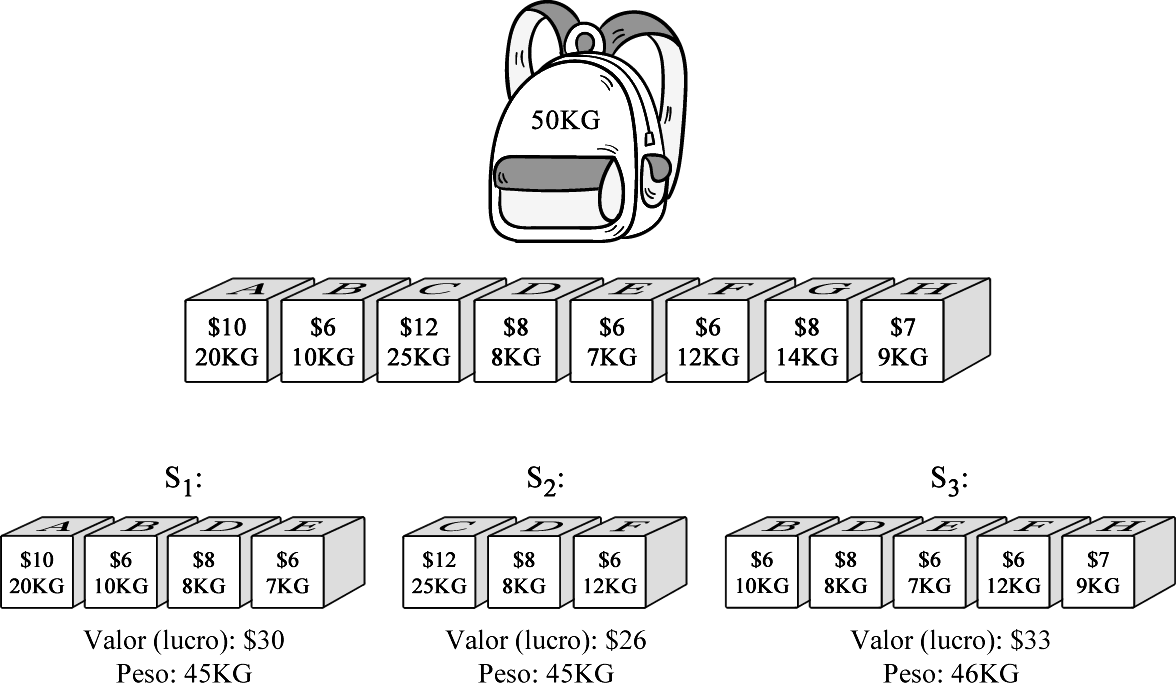
\includegraphics[width=1\textwidth]{cap_problemas/figs/mochila.png}
	\caption{\label{fig_knapsack}Exemplo para o problema da mochila mono-objetivo.}
\end{figure}

Na \autoref{fig_knapsack}, a capacidade máxima da mochila é 50Kg e existem oito itens disponíveis para se escolher. Três soluções possíveis são mostradas ($S_1$, $S_2$ e $S_3$), sendo que a melhor delas é $S_3$, pois possui o maior valor de lucro e ao mesmo tempo é válida, ou seja, respeita a restrição de capacidade (peso menor que 50Kg). No exemplo, todas as soluções estão saturadas, em outras palavras, a adição de qualquer outro item as tornam inválidas.

Existem diversas estratégias para resolver o \ac{PM}. Dentre elas, as mais usadas são os algoritmos gulosos \cite{KnapsackGreedy}, a programação dinâmica \cite{KnapsackDynamic} e os algoritmos genéticos \cite{KnapsackGA}. Os algoritmos gulosos e a programação dinâmica são os mais rápidos e eficientes para resolver o PM mono-objetivo. Em contrapartida, a complexidade adicionada ao considerar mais de um objetivo inviabiliza a utilização desse tipo de algoritmo, tornando os algoritmos genéticos e demais métodos bio-inspirados as melhores opções.

O problema da mochila multiobjetivo (PMM) é similar ao mono-objetivo (PM). Sua única diferença está no fato de que cada item, ao invés de possuir um único valor (lucro), é composto de múltiplos valores. No PMM, a função $lucro(o_i)$ retorna um vetor ao invés de um único valor escalar. Cada componente (elemento) do vetor representa o valor do item $o_i$ considerando um dos objetivos. Por exemplo, considerando um PMM de 3 objetivos, cada $o_i \in O$ possui um vetor formado por três valores de lucros (um para cada objetivo). O objetivo do problema passa a ser maximizar todos os lucros ao invés de um único valor. A definição do problema da mochila utilizada neste trabalho, também utilizada em \cite{MKP}, considera apenas um peso por item e uma única restrição, referente à capacidade da mochila. Outra definição mais comum do PMM envolve a consideração de múltiplos pesos por item e múltiplas restrições para a mochila, o número de pesos e de restrições é o mesmo que o número de objetivos. Essa definição alternativa é bastante comum na literatura e foi utilizada nos trabalhos de \cite{Alaya2004,Chu1998,Ishibuchi2015}. 

O PMM já foi utilizado várias vezes para avaliar algoritmos multiobjetivos, podendo-se destacar os trabalhos de \cite{Zitzler1999}, \cite{Zitzler2002} e \cite{Zhang2007}. As instâncias do PMM utilizadas no decorrer deste trabalho foram geradas de forma aleatória e compreendem problemas da mochila com 30, 40, 50, 100 e 200 itens. Para gerar as instâncias, sortearam-se valores no intervalo (0, 1000) para os lucros e para os pesos. A capacidade da mochila foi sempre definida como 60\% da soma dos pesos.

Uma das partes mais importantes de um algoritmo de busca bio-inspirado é a modelagem da solução. Para resolver o PMM através de algoritmos genéticos, é necessário definir a representação da solução, a geração aleatória de indivíduos, o cruzamento e a mutação. A representação de uma solução no AG para o problema da mochila mono-objetivo é simples, pois a solução é representada por um vetor binário e a literatura está repleta de exemplos que podem ser resolvidos dessa maneira \cite{KnapsackGA,Hristakeva2013}. A versão \textit{many-objective} do problema não requer modificação no modelo, fazendo com que os mesmos processos de cruzamento e mutação possam ser utilizados. Nas seções a seguir, detalhe-se a representação da solução e os operadores genéticos para o PMM usados neste trabalho. A construção das soluções nos algoritmos ACO é mais elaborada e será definida no próximo capítulo.

\subsection{Representação da solução e geração da população inicial}
\label{section_representacao_pmm}
Uma solução para o PMM é representada por um vetor binário. Se a instância do problema da mochila apresenta 10 itens ao total, por exemplo, um vetor com 10 bits representa a solução. As posições do vetor representam a ausência ou a presença de cada item. Se a posição $i$ do vetor é 0, então o $i$-ésimo item não faz parte da solução. Caso contrário, se o vetor na posição $i$ vale 1, então o  $i$-ésimo item está presente na mochila. Por exemplo, em uma solução representada pelo vetor [1,0,0,1,0,1,1,0,0,0], apenas os itens 0, 3, 5 e 6 são colocados na mochila, os outros itens (1, 2, 4, 7, 8 e 9) são descartados. Essa abordagem garante que cada solução possua uma única forma de representação, eliminando a característica multimodal do problema.

Nesse cenário, a geração aleatória de uma solução consiste em sortear os valores 0 ou 1 para cada posição do vetor. Tanto a geração aleatória de um indivíduo na formação da população inicial, quanto a combinação de vetores (cruzamento) não garantem a formação de uma solução válida, ou seja, é possível criar um vetor, cuja soma dos pesos dos itens ultrapasse a capacidade da mochila. Portanto, após a geração de qualquer solução, seja aleatória na população inicial ou proveniente de um \textit{crossover}, é necessário executar um processo de validação da solução. Para validar um vetor binário, basta verificar a soma dos pesos associados aos itens representados por 1. Caso esse valor seja maior que a capacidade da mochila, remove-se um item aleatório. Esse processo é repetido sucessivamente, até que a solução se torne válida, ou seja, até que a soma dos pesos dos itens respeite a capacidade da mochila \cite{Ishibuchi2015}.

\subsection{Cruzamento e mutação}
O cruzamento entre duas soluções binárias, como explicado na Seção \ref{section_ag}, pode ser efetuado de diversas maneiras. Neste trabalho, foi utilizado \textit{crossover} uniforme, ou seja, o filho herda de forma aleatória os bits do pai 1 ou do pai 2. Esse processo é ilustrado na \autoref{fig_cross_uniforme}.

\begin{figure}[!htbp]
	\centering
	\renewcommand{\arraystretch}{2} 
	\begin{tabular}{rl}
		Pai 1: & 
		\renewcommand{\arraystretch}{1.15} 
		\begin{tabular}{|c|c|c|c|c|c|}
			\hline 
			\rowcolor[HTML]{F5D1CF}
			0 & 0 & 1 & 0 & 1 & 1 \\
			\hline 
		\end{tabular}
		\\
		Pai 2: & 
		\renewcommand{\arraystretch}{1.15} 
		\begin{tabular}{|c|c|c|c|c|c|}
			\hline 
			\rowcolor[HTML]{CCCCFF}
			1 & 0 & 0 & 1 & 1 & 0 \\
			\hline 
		\end{tabular}
		\\
		Máscara: & 
		\renewcommand{\arraystretch}{1.15} 
		\begin{tabular}{|c|c|c|c|c|c|}
			\hline 
			0 & 1 & 0 & 0 & 1 & 0 \\
			\hline 
		\end{tabular}
		\\
		Filho 1: & 
		\renewcommand{\arraystretch}{1.15} 
		\begin{tabular}{|c|c|c|c|c|c|}
			\hline 
			\cellcolor[HTML]{F5D1CF}0 & \cellcolor[HTML]{CCCCFF}0 & \cellcolor[HTML]{F5D1CF}1 & \cellcolor[HTML]{F5D1CF}0 & \cellcolor[HTML]{CCCCFF}1 & \cellcolor[HTML]{F5D1CF}1 \\
			\hline 
		\end{tabular}
		\\
		Filho 2: & 
		\renewcommand{\arraystretch}{1.15} 
		\begin{tabular}{|c|c|c|c|c|c|}
			\hline 
			\cellcolor[HTML]{CCCCFF}1 & \cellcolor[HTML]{F5D1CF}0 & \cellcolor[HTML]{CCCCFF}0 & \cellcolor[HTML]{CCCCFF}1 & \cellcolor[HTML]{F5D1CF}1 & \cellcolor[HTML]{CCCCFF}0 \\
			\hline 
		\end{tabular}
	\end{tabular}
	\caption{\label{fig_cross_uniforme}Exemplo de crossover uniforme}
\end{figure}

Como pode ser visto na Figura \ref{fig_cross_uniforme}, o \textit{crossover} uniforme pode ser implementado com uma máscara, que é um vetor aleatório de bits que controla os genes herdados de cada pai. Se o bit na posição $i$ da máscara vale 0, então o gene do filho na posição $i$ herda o valor de um dos pais (ex: pai 1), caso contrário, herda o valor do outro (ex: pai 2). Dessa forma, ainda é possível gerar 2 filhos: um deles usando a regra na qual o bit 0 da máscara representa o pai 1 e o bit 1 representa o pai 2 (filho 1 na figura); e o outro usando a máscara com os valores complementares (filho 2).

Após o \textit{crossover}, existe uma chance, determinada pela taxa de mutação definida para o AG, do indivíduo sofrer alguma mutação genética. Neste trabalho, foi utilizado o método mais simples de mutação para vetores binários, ou seja, a inversão de bit. Esse processo consiste em sortear uma posição aleatória do vetor e se o valor for 0, troca-se para 1, caso contrário, troca-se para 0.

\section{Problema do roteamento multicast}
\label{section_problemas_prm}

\subsection{Definição do problema}

O problema do roteamento multicast (PRM) aparece na engenharia de tráfego em redes de computadores e consiste em escolher a forma ``mais eficiente'' de transmitir uma mensagem multicast \cite{Lafeta2016}. Uma transmissão de rede pode ser do tipo unicast, multicast ou broadcast. Em transmissões unicast, conecta-se um ponto da rede a outro ponto qualquer (transmissão ponto-a-ponto). Para fazer isso de forma eficiente, é possível usar algum algoritmo capaz de encontrar o melhor caminho entre os dois pontos (e.g. \cite{Dijkstra1959}), se apenas uma métrica for utilizada. As comunicações broadcast caracterizam-se pelo fato de um nó da rede (servidor) enviar o conteúdo a todos os demais. Para obter as melhores rotas para trafegar os dados, é possível utilizar algum algoritmo capaz de determinar a árvore geradora de custo mínimo (e.g. \cite{Prim1957}), se apenas uma métrica for empregada na otimização. Em uma comunicação multicast, o objetivo é transmitir o conteúdo de um nó da rede, chamado nó de origem ou transmissor, para alguns outros nós, denominados receptores. Essa tarefa apresenta maior complexidade, mesmo no caso de uma única métrica, pois é necessário obter uma árvore de Steiner de custo mínimo, o que é mais difícil que calcular uma única rota ou construir a árvore geradora de custo mínimo \cite{Bueno2010}.

O PRM é um problema prático muito importante. Seu estudo visa o desenvolvimento de algoritmos eficientes e eficazes, proporcionando avanços na geração de rotas em redes de computadores. O objetivo desses algoritmos é encontrar soluções (rotas multicast) que permitam uma comunicação mais rápida, menos custosa e mais confiável entre dispositivos, o que é essencial em uma era onde a maioria das pessoas consomem informação e entretenimento pela Internet.

Uma vez que se deseja transmitir um conteúdo via uma rede de computadores, o problema, em sua versão com um único objetivo de custo, consiste em encontrar a melhor rota possível entre a fonte de dados e os vários destinos. Dado um grafo $G=(V,E)$, que representa a rede de comunicação, um nó raiz $r \in V$ (nó transmissor) e um conjunto de nós destinos $D \subset V$ (nós receptores), o PRM consiste em determinar a subárvore $T$ de $G$ enraizada em $r$ que inclui todos os vértices em $D$ e apresenta o menor custo possível. A \autoref{fig_prm_grafo} ilustra uma instância do problema de roteamento multicast. Nesse exemplo de rede de comunicação, o nó transmissor é definido por um círculo duplo (vértice 0), os nós receptores são destacados em cinza escuro (vértices 1, 8, 12 e 13) e os nós intermediários estão em cinza claro. Os números em cada aresta determinam o custo da comunicação entre os nós que ela conecta.

\begin{figure}[!htbp]
	\centering
	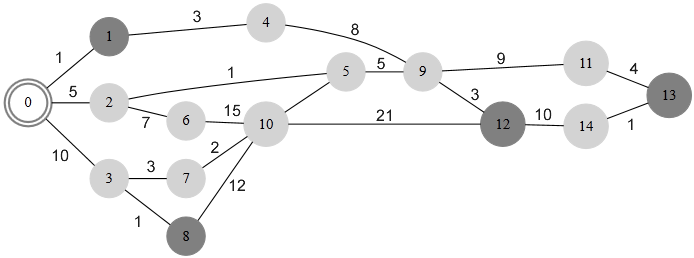
\includegraphics[width=1\textwidth]{cap_problemas/figs/prm_grafo}
	\caption{\label{fig_prm_grafo}Exemplo de uma rede de comunicação. Retirado de \cite{BuenoThesis}.}
\end{figure}

Na \autoref{fig_prm_mono}, são apresentados alguns exemplos de árvores multicast criadas a partir do grafo mostrado na figura \autoref{fig_prm_grafo}. O custo de cada árvore é dado pela soma dos custos de suas arestas. Dentre os exemplos, a árvore mais à direita possui o menor custo total: 65.

\begin{figure}[!htbp]
	\centering
	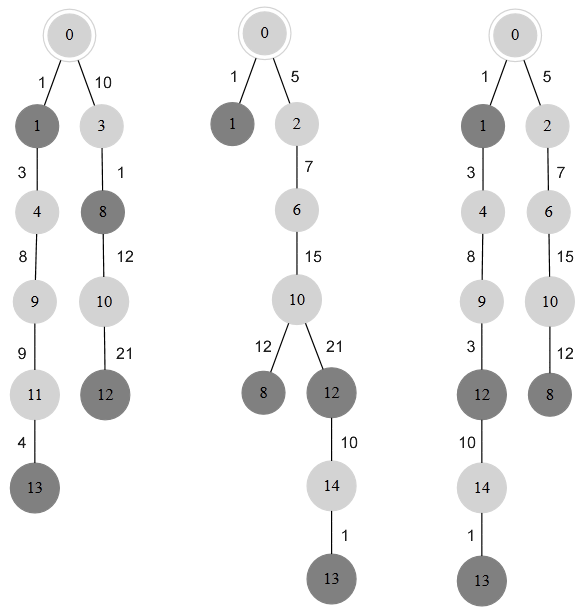
\includegraphics[width=0.8\textwidth]{cap_problemas/figs/prm_mono}
	\caption{\label{fig_prm_mono}Exemplos de árvores multicast relativos ao grafo da figura \autoref{fig_prm_grafo}. Retirado do trabalho de \cite{LafetaThesis}}
\end{figure}

O PRM original é proposto com apenas um objetivo a se otimizar e utiliza uma métrica por enlace, que é o custo. Essa métrica pode representar uma combinação de outras métricas. Entretanto, áreas que tratam da melhoria do desempenho em redes de computadores, como a engenharia de tráfego e a \ac{QoS} trouxeram uma nova necessidade para a transmissão em redes, onde a utilização de métricas distintas é mais adequada ao gerenciamento da rede. Características como distância, atraso (\textit{delay}), capacidade de tráfego e uso do tráfego são boas métricas da qualidade de serviço (QoS) em uma comunicação \cite{LafetaThesis}. Nesse contexto, este trabalho investiga uma versão multiobjetivo do problema de roteamento multicast. Nesta versão do problema, as árvores apresentadas como solução devem representar o melhor compromisso entre as métricas utilizadas.

\begin{figure}
	\centering
	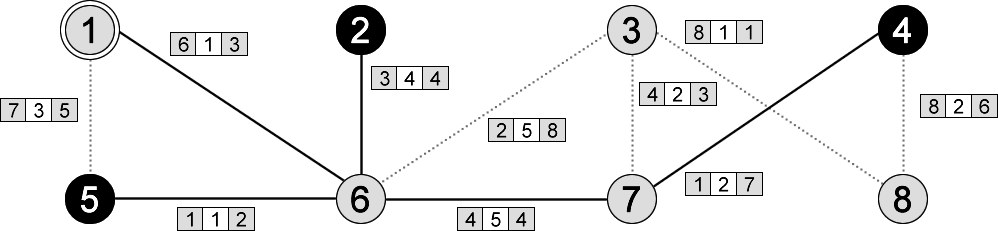
\includegraphics[width=1\textwidth]{cap_problemas/figs/prm_multi}
	\caption{\label{fig_prm_multi}Exemplo de árvore multicast no PRM multiobjetivo.}
\end{figure}

Na \autoref{fig_prm_multi} é apresentado um exemplo de rede com as métricas ``custo'' (primeiro valor), ``delay'' (segundo valor) e ``tráfego corrente'' (terceiro valor) nas arestas. As arestas representadas por linhas contínuas identificam uma árvore multicast ótima (não-dominada) para os objetivos ``custo total'', ``delay-fim-a-fim médio'' e ``utilização média dos enlaces'', descritos mais a frente no texto. Na figura, o nó 1 é a raiz e os nós com fundo escuro representam os nós destinos. Para esse exemplo, no objetivo ``utilização média dos enlaces'', considerou-se a mesma capacidade de tráfego para todos os enlaces, de forma que apenas o tráfego corrente fosse relevante.

Neste trabalho consideram-se até quatro valores de peso para um enlace da rede: custo, \textit{delay}, capacidade de tráfego e tráfego corrente, representados respectivamente pelas funções: $c()$, $d()$, $z()$ e $t()$. Por meio dessas medidas são formulados os seguintes objetivos:

\begin{enumerate} 
	\item \textbf{Custo total:} soma dos valores de custo de todas as arestas da árvore.
	\item \textbf{Delay fim-a-fim médio:} média da soma dos \textit{delays} em cada ramo da árvore. Em outras palavras, média do atraso em cada uma das comunicações cliente-servidor.
	\item \textbf{Delay fim-a-fim máximo:} maior valor para a soma de \textit{delays} dentre todos os ramos da árvore, ou seja, o maior atraso dentre todas as comunicações cliente-servidor.
	\item \textbf{\textit{Hops count}}: número de vértices na árvore.
	\item \textbf{Utilização máxima de enlaces:} considerando todas as arestas na árvore, qual delas atinge a maior utilização de banda? Matematicamente, considerando $E$ o conjunto de arestas da árvore e $\phi$ o tamanho da mensagem, essa métrica é dada por:
	\begin{equation}\max_{e \in E} \frac{t(e) + \phi}{z(e)}\end{equation}
	\item \textbf{Utilização média dos enlaces:} média da utilização de banda entre todas as arestas da árvore. Seu cálculo é similar ao da métrica anterior (utilização máxima de enlaces) e é dado por:
	\begin{equation}\frac{\sum_{e \in E} \frac{t(e) + \phi}{z(e)}}{|E|}\end{equation}
\end{enumerate}

A fim de possibilitar diversos cenários de teste para o PRM, os objetivos acima podem ser combinados de diversas maneiras, criando várias instâncias multiobjetivo do problema. Neste trabalho foram utilizadas 5 formulações (combinações) desses objetivos:

\begin{enumerate}
	\item $P_2$: formado pelos objetivos 1 e 3.
	\item $P_3$: formado pelos objetivos 1, 3 e 4.
	\item $P_4$: formado pelos objetivos 1, 3, 4 e 5.
	\item $P_5$: formado pelos objetivos 1, 3, 4, 5 e 6.
	\item $P_6$: formado pelos objetivos 1, 2, 3, 4, 5 e 6.
\end{enumerate}

Essas combinações de objetivo foram formuladas em trabalhos anteriores \cite{LafetaThesis,BuenoThesis} e, segundo esses estudos prévios, apresentam baixo grau de correlação. Ou seja, um problema de 6 objetivos realmente representa 6 variáveis distintas, onde uma não pode ser calculada como função da outra.

O PRM foi trabalhado sobre 5 redes diferentes variando a complexidade em termos de quantidade de nós destinos, vértices e arestas. Essas redes foram retiradas do trabalho de \cite{Lafeta2016} e suas caraterísticas são apresentadas na Tabela \ref{tab_prm_redes}.

\begin{table}[!htbp]
	\centering
	\caption{Definições das redes utilizadas no PRM}
	\label{tab_prm_redes}
	\begin{tabular}{r|rrr}
		Nome        & Destinos & Vértices & Arestas \\ \hline
		Rede 1 (R1) & 10       & 33       & 106     \\
		Rede 2 (R2) & 18       & 75       & 188     \\
		Rede 3 (R3) & 37       & 75       & 188     \\
		Rede 4 (R5) & 12       & 75       & 300     \\
		Rede 5 (R5) & 16       & 100      & 250     \\ \hline
	\end{tabular}
\end{table}

Para resolver o PRM através de estratégias evolutivas, é necessário, em primeiro lugar, definir a modelagem do indivíduo. Esse processo não é muito simples, pois a solução não pode ser representada por um vetor. De fato, como deve representar os caminhos entre o servidor e os múltiplos destinos em uma rede de computadores, a solução para o PRM é melhor representada por uma árvore. Dessa forma, é preciso desenvolver o processo de crossover e de mutação de acordo com essa estrutura. O operador de cruzamento deve receber duas árvores pais e gerar uma nova árvore (filha) que compartilha características de ambos os pais. O operador de mutação precisa criar uma pequena alteração na árvore que permita explorar diferentes regiões do espaço de busca, mas que não a descaracterize completamente. As seções a seguir apresentam o modelo adotado nas abordagens evolutivas para o PRM.

\subsection{Representação da solução}

Como mostrado na seção \ref{section_problemas_prm}, considerando que em cada nó da rede a mensagem pode ser replicada e enviada aos próximos nós conectados, o PRM deseja encontrar a árvore que representa o processo de transmissão de menor custo que parte do nó fonte (servidor) e atinge todos os destinos. Existem duas maneiras de se representar uma solução:

\begin{enumerate}
	\item \textbf{Representação em árvore:} \cite{Bueno2010} o AG evolui a própria árvore que se deseja encontrar como solução. É um processo mais complicado que elimina a necessidade de pós-processamento. A \autoref{fig_prm_mono}, mostra alguns exemplos de árvores multicasts.
	\item \textbf{Representação em conjunto:} \cite{Baran2004} o AG evolui um conjunto de caminhos $C$, ou seja, para cada nó destino $d$, deve existir uma sequência de nós $L \in C$ que contém o caminho que leva do nó servidor (emissor) até o nó $d$. A representação em conjuntos de caminhos é mais fácil de se gerenciar, mas exige a transformação (conjunção) dos caminhos pertencentes ao conjunto em uma árvore  ao final do processo. Como diferentes árvores podem ser formadas a partir de um único conjunto de caminhos, essa representação não é tão eficiente quanto a anterior ao explorar o espaço de busca.
\end{enumerate}

Neste trabalho, optou-se por utilizar a representação em árvores.

\subsection{Geração da população inicial}

Considere um grafo da rede $G$, um nó raiz (também chamado de servidor ou emissor) $r$ e um conjunto de nós de destino $D$. Para criar uma solução aleatória no PRM, inicia-se um grafo $S$ apenas com o vértice $r$. O passo seguinte é extrair um destino aleatório $d \in D$ e, com base no grafo $G$, criar um caminho em $S$ entre qualquer um de seus vértices atuais e $d$. Após construir o caminho, $d$ com certeza será atingível a partir de qualquer vértice de $S$. O processo se repete até que todos os nós destinos estejam no grafo $S$. Por fim, o grafo $S$ é transformado em uma árvore a partir da remoção dos ciclos presentes em $S$ e da aplicação de podas dos ramos desnecessários.

Para criar o caminho aleatório entre um vértice de $S$ e um nó destino $d$, considera-se um vetor de exploração $Exp$ que, inicialmente, contém todos os nós de $S$. Enquanto o destino $d$ não é encontrado, algum nó $exp_i \in Exp$ é escolhido e todos os vértices adjacentes (conectados) a $exp_i$ são incluídos em $Exp$. Quando $d$ é encontrado, adiciona-se a $S$ o caminho necessário para sair de algum vértice de $S$ e chegar ao destino $d$.

\subsection{Cruzamento}

A estratégia de cruzamento utilizada neste trabalho para o PRM é chamada de cruzamento por caminho e foi proposta em \cite{Lafeta2016} como alternativa ao cruzamento por similaridade utilizado em trabalhos anteriores \cite{Bueno2010}. Esse tipo de cruzamento é realizado entre duas árvores $P_1$ e $P_2$ e produz um único filho $F$. O processo consiste em separar cada um dos pais em ramos e, então, para cada nó destino $d$, acrescentar a $F$ o ramo de $P_1$ ou de $P_2$ que leva a $d$. A escolha entre $P_1$ e $P_2$ é feita de forma aleatória. Assim que todos os nós destinos são atingíveis em $F$, a etapa de seleção de ramos é interrompida, os ciclos que possivelmente foram criados são removidos, e um processo de poda é realizado a fim de remover qualquer nó folha que não seja destino.

\begin{figure}[!htbp]
	\centering
	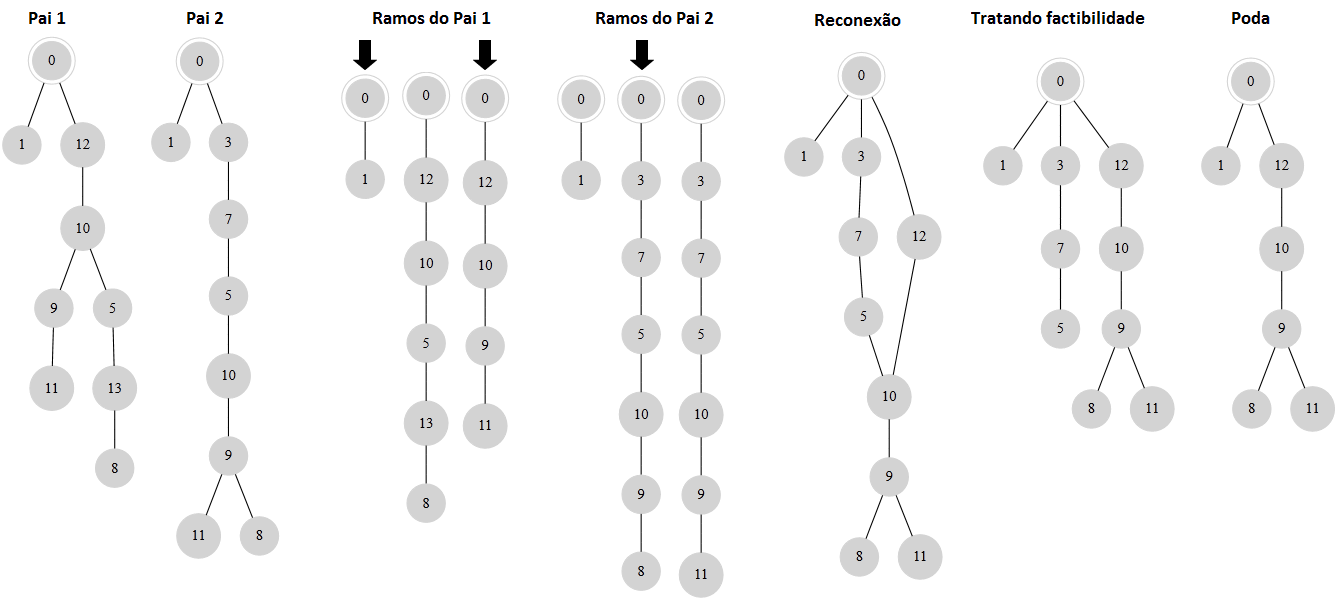
\includegraphics[width=1\textwidth]{cap_problemas/figs/prm-cruzamento-caminho}
	\caption{\label{fig_prm-cruzamento-caminho}Exemplo de cruzamento por caminho, onde o nó raiz é 0 e os destinos são \{1, 8, 11\}. Retirado de \cite{LafetaThesis}}
\end{figure}

A \autoref{fig_prm-cruzamento-caminho} representa o processo de cruzamento por caminho entre duas árvores (Pai 1 e Pai 2). No exemplo, o nó raiz é o vértice 0 e os nós destinos são o conjunto $\{1, 8, 11\}$. As setas em ``ramos do pai 1'' e ``ramos do pai 2'' representam os caminhos escolhidos em cada um dos pais para compor a árvore filha. O grafo nomeado ``reconexão'' representa o filho após a inclusão de todos os ramos. Como foi gerado um ciclo (existem dois caminhos da origem até o nó 10), o mesmo deve ser removido a fim de obter uma árvore válida. Supondo que o caminho $0 \rightarrow 12 \rightarrow 10$ tem menor custo que o caminho $0 \rightarrow 3 \rightarrow 7 \rightarrow 5 \rightarrow 10$, o nó 10 será acessado apenas a partir do nó 12. Em ``tratando factibilidade'', apresenta-se o filho após a remoção dos ciclos. Como os nós 3, 7 e 5 não são destinos, eles são removidos durante o processo de poda, resultando na última árvore (``poda'') que é o filho.

Para remover os ciclos, percorre-se a árvore em largura removendo qualquer aresta que adicione ciclo. No processo de poda, verificam-se todas as folhas. Se algum nó folha não for um destino, ele é removido e o processo repetido até que todos os nós folhas sejam destinos.

Após o cruzamento, realiza-se um processo de filtragem, onde todas as soluções repetidas são substituídas por novos indivíduos gerados aleatoriamente.

\subsection{Mutação}

A mutação em uma árvore que representa uma solução para o PRM consiste em remover parte dos nós da árvore e então reconectá-los de maneira aleatória utilizando o grafo correspondente à rede em questão. As etapas desse processo estão descritas no algoritmo \ref{alg_prm_mutacao}.

\begin{algorithm}
	\caption{Mutação para uma árvore $(A, G, qte_{arestas}, r, D)$}
	\label{alg_prm_mutacao}
	\begin{algorithmic}[1]
		\State desconectar($A$, $qte_{arestas}$)
		\State $C \gets extraiComponente(A, r)$
		\State $M \gets novoGrafo()$
		\State $M \gets mesclar(M, C)$
		\While{$|D| > 0$}
		\State $d \gets removeAleatorio(D)$
		\State $C \gets extraiComponente(A, d)$
		\If{$d \notin V(M)$}
		\State $P \gets caminhoAlearorio(C, M, G)$
		\State $M \gets mesclar(M, P)$
		\EndIf
		\State $M \gets mesclar(M, C)$
		\EndWhile
		\State $removerCiclos(M)$
		\State $podarArvore(M)$
		\State \Return $M$
	\end{algorithmic}
\end{algorithm}

O algoritmo recebe como entrada a árvore que sofrerá mutação ($A$), o grafo da rede ($G$), a quantidade de arestas a se remover na mutação ($qte_{arestas}$), o vértice raiz ($r$), e o conjunto de destinos ($D$). Na linha 1, desconecta-se a árvore através da remoção aleatória de $qte_{arestas}$ arestas. Entre as linhas 2 e 4, cria-se a estrutura para a construção da árvore ($M$). A partir da linha 5 começa o laço para reconectar todos os nós destinos à arvore. A linha 6 seleciona um destino aleatório $d$ para reconectar. Na linha 7, a componente conexa contendo $d$ é extraída de $A$ e chamada de $C$. Se não existe componente conexa com o vértice $d$, $C$ será um grafo com um único nó ($d$) e nenhuma aresta. Caso o vértice $d$ não exista na componente conexa $M$, cria-se um caminho aleatório em $M$ (com base no grafo $G$) que a conecta a $C$ (linhas 8 a 10). A construção do caminho aleatório é feita nó a nó até se encontrar uma sequência de arestas entre as duas componentes. Na linha 12, incluem-se em $M$ todas as arestas de $C$. Ao final, o mesmo pós-processamento do cruzamento por caminho é realizado: remoção de ciclos e poda da árvore (linhas 14 e 15).

Em relação à proposta utilizada em \cite{LafetaThesis}, destacam-se como diferenças a geração da população inicial e o cruzamento. Com relação à população inicial, os indivíduos gerados através do método descrito neste trabalho apresentam diversidade um pouco maior. No que diz repeito ao cruzamento, aqui se utiliza apenas o \textit{crossover} por caminho, enquanto no trabalho anterior se utilizava também um outro tipo de cruzamento, o \textit{crossover} por similaridade.